\section{Alpha Particle Formation in Neutron Rich Matter}
\red{Include theory here and then talk about the results\\}
\blue{Talk about the limitations of momentum ``shells" that must be filled. Mention the possible use of ``twist" boundary conditions in the future.\\}
\red{Talk also about why you did both linear and quadratic, etc.\\}
One of the triumphs of nuclear physics is the ability to describe properties of macroscopic systems such as neutron stars with microscopic interactions. Neutron stars have been studied extensively with QMC methods from the nuclear EOS \cite{sarsa2003,gandolfi2014} to the hyperon problem \cite{lonardoni2015,gandolfi2018}. As the density of nuclear matter increases the choice of the 3N force becomes more important. However, for neutron star crusts with densities only up to about 0.5$\rho_0$ the choice of 3N force is not as crucial, and NN forces alone can give good results. The outer crusts of neutron stars host atom nuclei in a degenerate bath of electrons. As the density increases inside the neutron star the nuclear binding force will eventually give way to neutron drip and the remaining nuclei will be in a fluid of dripped neutrons. This has been studied \cite{lorenz1993,chamel2015} and the density at which neutron rich nuclei begin to drip neutrons is about $\rho_\text{drip} = 4.3\times10^{11}$ g cm$^{-3}$ or 0.00026 fm$^{-3}$. This neutron drip will leave smaller and smaller nuclei in a sea of neutrons. At some point even the smallest nuclei will dissolve to form uniform neutron matter, or mostly-neutron matter. To investigate this transition I have studied the formation of alpha particles in mostly-neutron matter. To do this I have used the AFDMC method in conjunction with the AV6$'$ potential using both the linear and quadratic trial wave functions. The energy of an alpha particle that has formed in neutron matter with an additional two protons would be
\begin{equation}
   E_\alpha = E_\text{Nn2p} - E_\text{Nn},
   \label{equ:alphaenergy}
\end{equation}
where $E_\text{Nn2p}$ is the energy for $N$ neutrons and 2 protons and $E_\text{Nn}$ is the energy for $N$ neutrons alone. I have calculated the energy per particle of 14 neutrons with and without the presence of 2 protons in a box with periodic boundary conditions. At proper densities the 2 protons will form, with 2 neutrons, an alpha particle surrounded by free neutrons and the energy of $E_\alpha$ in Equation~\ref{equ:alphaenergy} will be the energy of the 2 protons and 2 neutrons. If the energy per particle is given by $\epsilon = E/A$ then for 14 neutrons this becomes
\begin{equation}
   E_\alpha = 14\epsilon_\text{14n2p} - 12\epsilon_\text{14n}.
   \label{equ:alphaenergy14n2p}
\end{equation}
I have plotted this energy as a function of density using both linear and quadratic correlations in Figure~\ref{fig:alpha}.
\begin{figure}[h!]
   \centering
   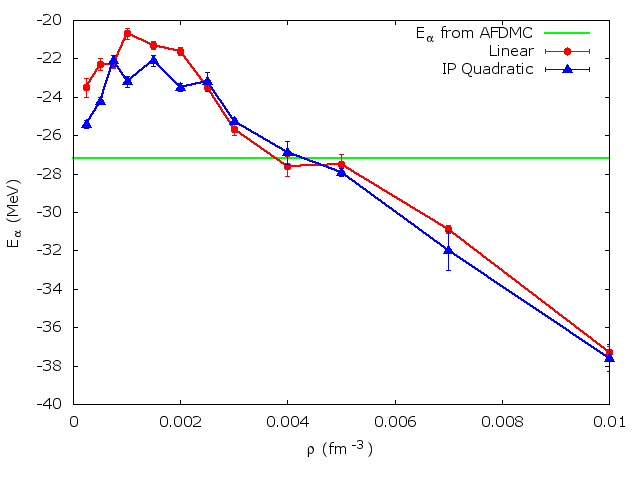
\includegraphics[width=0.7\textwidth]{figures/alpha.png}
   \caption{Energy of 2 protons and 2 neutrons with 12 free neutrons as calculated with Equation~\ref{equ:alphaenergy14n2p} as calculated with linear and quadratic correlations. I have also added a green horizontal line at the alpha particle energy as calculated with AFDMC using the same AV6$'$ interaction and quadratic correlations.}
   \label{fig:alpha}
\end{figure}
If the free neutrons did not interact with the formed alpha particle it would be expected that the alpha particle energy would agree with previous AFDMC calculations. At densities below 0.0025 fm$^{-3}$ the alpha particle is underbound by a few MeV for both linear and quadratic correlations. The quadratic correlations do decrease the alpha energy at low densities. The energy for each individual calculation of $\epsilon_\text{14n2p}$ and $\epsilon_\text{14n}$ were decreased with quadratic correlations with respect to linear correlations. The difference between quadratic and linear correlations seems to be the most important for most densities below 0.0025 fm$^{-3}$.

The discrepancy in alpha particle energy at low densities then must be due to the excess neutrons deforming the alpha particle. To verify that 2 protons and 2 neutrons will give the correct energy when put in a box I have calculated the energy of 2 protons and 2 neutrons in various boxes of different densities as shown in Figure~\ref{fig:alpha2n2p}.
\begin{figure}[h!]
   \centering
   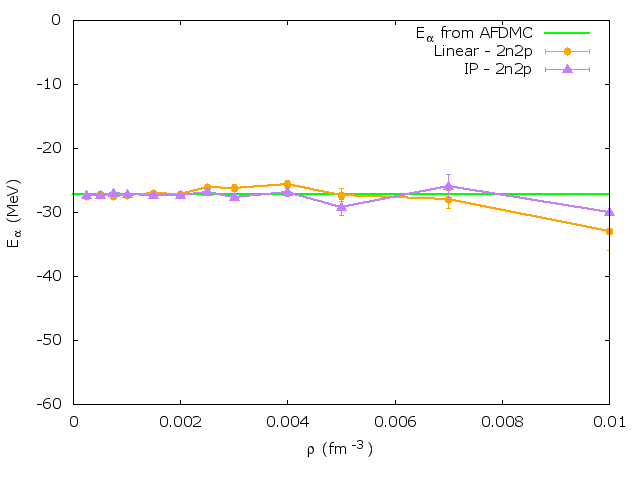
\includegraphics[width=0.7\textwidth]{figures/2n2p.png}
   \caption{Energy of 2 protons and 2 neutrons with 12 free neutrons as calculated with Equation~\ref{equ:alphaenergy14n2p} as calculated with linear and quadratic correlations. I have also added a green horizontal line at the alpha particle energy as calculated with AFDMC using the same AV6$'$ interaction and quadratic correlations.}
   \label{fig:alpha2n2p}
\end{figure}
The energy at low densities is much closer to the alpha particle energy as calculated with AFDMC.

The other possible explanation for the difference in energy is that an alpha particle isn't forming at all. To investigate this I have looked at the pair correlations function
\begin{equation}
   g_\mathcal{O}(r) = \frac{1}{4\pi r^2} \bra{\Psi}\sum\limits_{i<j}\mathcal{O}_{ij}\delta(r-r_{ij})\ket{\Psi},
\end{equation}
where I have specifically looked at the case where the operator is the $pp$ operator. The $g_{pp}(r)$ distribution gives the probability of finding two protons at a distance $r$ from each other. I have plotted these for a few of the densities for which energies were calculated in Figure~\ref{fig:gpp}.
\begin{figure}[h!]
   \centering
   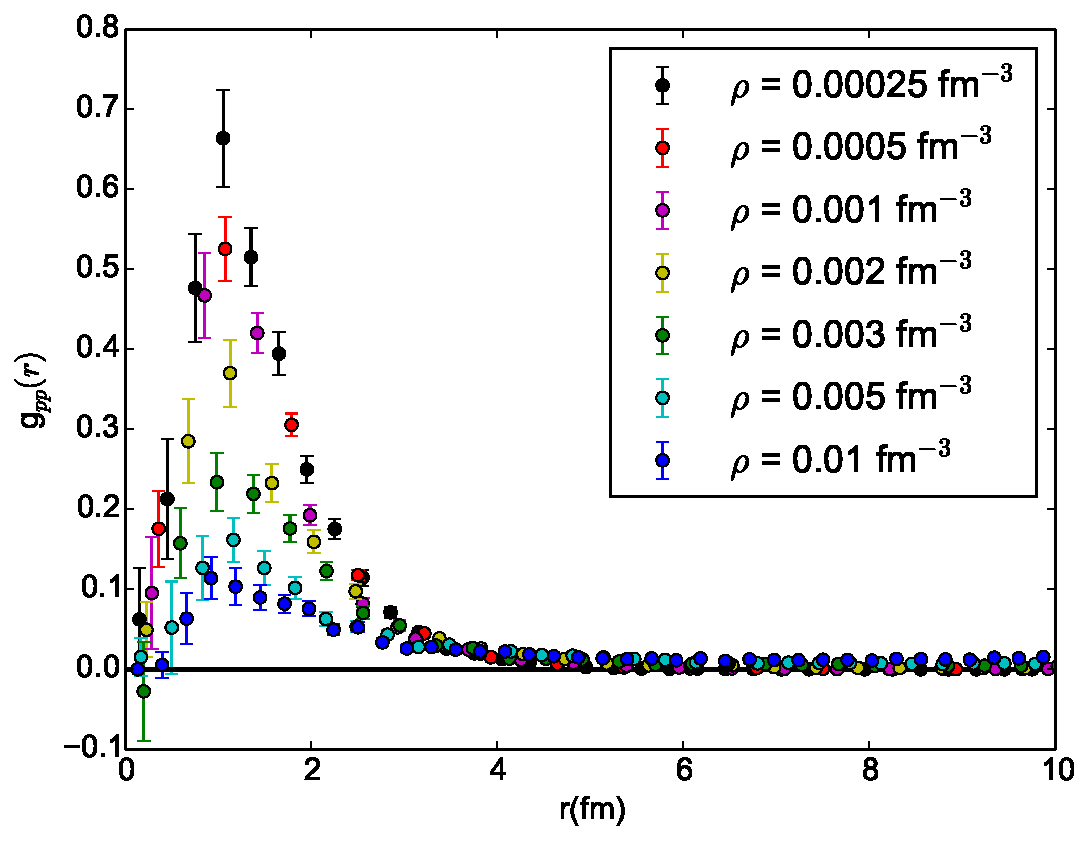
\includegraphics[width=0.7\textwidth]{figures/gpp.pdf}
   \caption{Pair correlations functions, $g_{pp}$ that give the probability of finding 2 protons a distance $r$ from each other. This is only shown for a few of the densities calculated to keep the figure less busy.}
   \label{fig:gpp}
\end{figure}
It is clear to see that as the density decreases the probability of finding the 2 protons at a close distance to each other increases. This is consistent with the formation of an alpha particle. The opposite is true, that as the density increases the protons are more likely to be found separated at larger distances, indicating the dissipation of the alpha particle. This can be seen in Figure~\ref{fig:gpp_small} which is simply showing more detail to the high separation tail in Figure~\ref{fig:gpp}
\begin{figure}[h!]
   \centering
   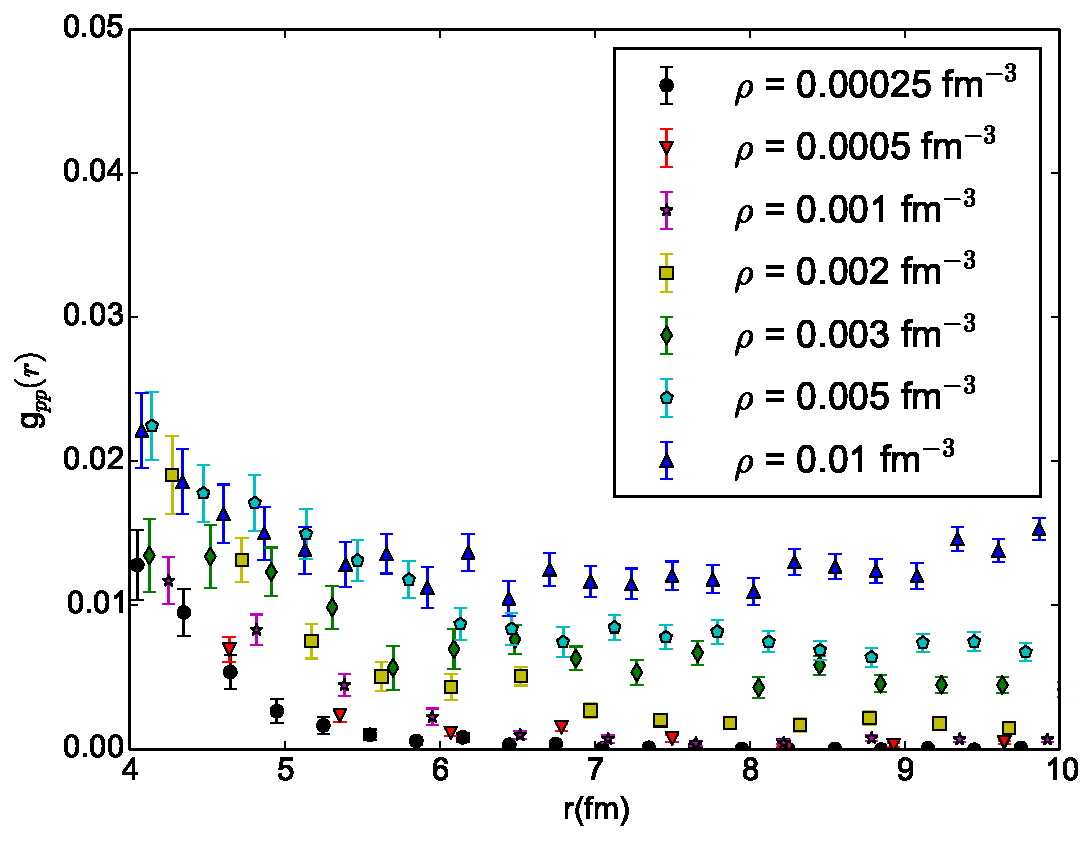
\includegraphics[width=0.7\textwidth]{figures/gpp_small.pdf}
   \caption{Large seperation part of the pair correlations functions $g_{pp}$ at different densities.}
   \label{fig:gpp_small}
\end{figure}

This provides good evidence that an alpha particle is forming at low densities. I have also calculated the pair distribution function for the alpha particle as calculated in the continuum, as opposed to the periodic box. In Figure~\ref{fig:fig:gpp_compare} I have plotted this against the $g_{pp}$ pair distribution functions for the 14 neutrons with 2 protons at $\rho=0.00025$ fm$^{-3}$ as calculated with both linear and quadratic correlations. I have increased the resolution of the $g_{pp}$ calculation to show more detail.
\begin{figure}[h!]
   \centering
   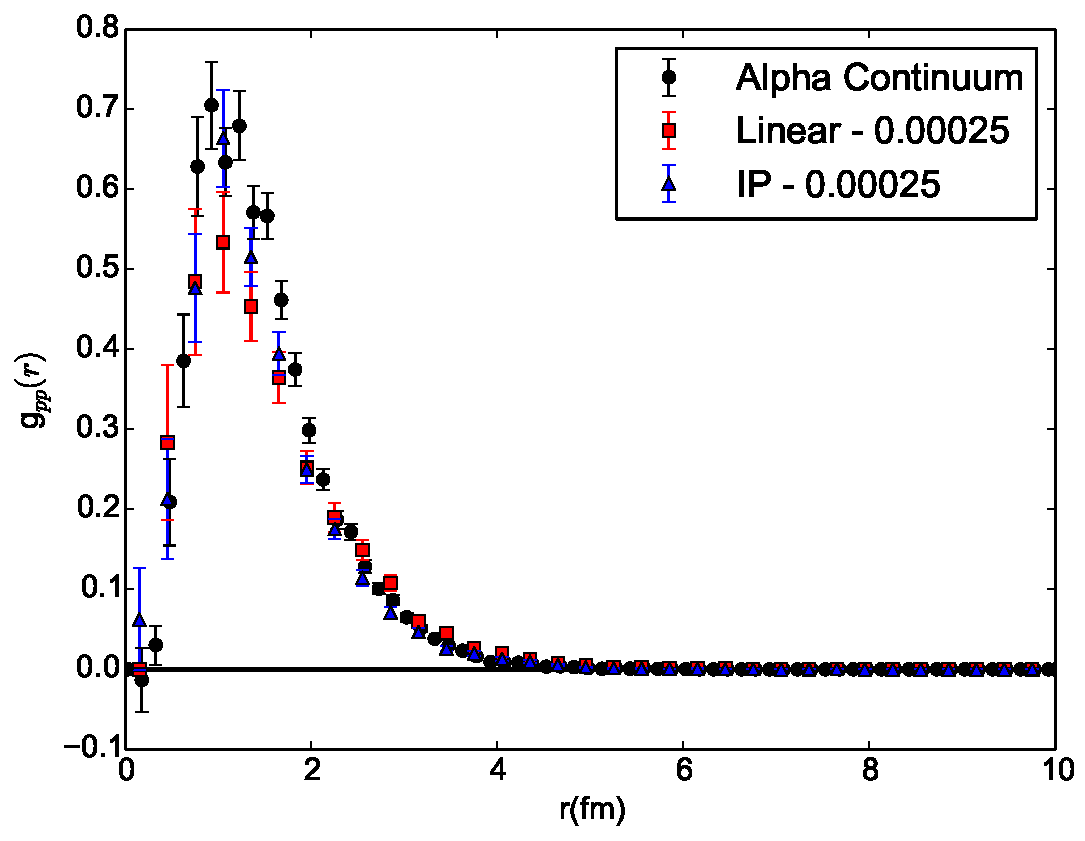
\includegraphics[width=0.7\textwidth]{figures/gpp_compare.pdf}
   \caption{Proton-proton pair distribution functions calculated in the continuum compared to the equivalent calculation a periodic box with $\rho=0.00025$ fm$^{-3}$. The $g_{pp}$ calculations in the box are increased resolution from those in earlier plots to show more detail. Both linear and IP quadratic correlations were used for the calculations in a box.}
   \label{fig:gpp_compare}
\end{figure}
As was seen before both the linear and IP quadratic correlations seem to be forming an alpha particle, but the IP quadratic correlations provide a much better fit to the pair correlation function of the alpha particle as calculated in the continuum.
